\documentclass[12pt]{article}
\usepackage{graphicx}

\begin{document}
\title{Adversarial Neural Cryptography}
\author{Michael Guarino\\
        Marist College Department of Computer Science\\
        MSCS 630: Security Algorithms and Protocols}
\maketitle
\begin{abstract}
Neural networks have been proven to be universal function approximators and therefore can learn to represent a great variety of functions given appropriate parameters. This property makes neural networks excellent candidates as encryption algorithms. Due to recent advancements in quantum computing technology, research in the area of non-conventional cryptographic methods is of vital importance as current cryptographic algorithms will likely be completely obsolete. This work looks to build on the Google Brain paper "Learning to Protect Communications with Adversarial Neural Cryptography" through exploring the novel use of neural networks in the area of symmetric encryption systems and to improve the original adversarial architecture proposed in Adbadi, et al. [1].
\end{abstract}

\section{Introduction}

Cryptography is concerned with algorithms and protocols that protect the secrecy of source information as it is transferred from it's point of origin to it's intended destination. Encryption describes the method used to convert source data or plaintext from an intelligible form to an encoded form by which can only be made intelligible through decoding the encoded form with access to a decryption key. An encryption algorithm is said to be secure if information about the plaintext cannot be extracted from cipher texts.
Neural networks have been proven to be universal function approximators and therefore can learn to represent a great variety of functions given appropriate parameters thus neural networks are excellent candidates as encryption algorithms. There has been some work in the area of using deep learning architectures to learn to encrypt source data; however, applications of deep learning in the area of cryptography have been largely unexplored.
The Google Brain paper "Learning to Protect Communications with Adversarial Neural Cryptography" introduces an symmetric encryption system that consists of neural networks named Alice and Bob whose goal is to communicate while limiting what a third neural network, Eve, can learn from eavesdropping on their communication [1]. Alice and Bob are trained adversarily to defeat Eve without a pre-specificed notion of what cryptosystem they may discover to accomplish this goal [1].

Generative adversarial networks (GAN) are a generative model devised by Goodfellow et al. in 2014 [2]. The GAN architecture is characterized by two differentiable functions, neural networks, that play different roles in refining the system. One differentiable function is known as the generator and the other is the discriminator. The generator learns to produce data from a learned probability distribution. The discriminator determines if the data that was produced by the generator is valid by determining if the input comes from the generator or from the actual data set. In this work we will validate that a generative adversarial network can be used to learn symmetric encryption specifically shared-key encryption.

The GAN architecture is known to be difficult to train being characterized as largely unstable for many reasons [4,5,6] the observation being that gradient descent used to update the parameters of the generator and discriminator are inappropriate when the solution to the optimization problem posed by GAN training actually constitutes a saddle point [3]. Recently there has been great improvements in theoretical explanation of GANs, improved GAN architectures, and training tricks to ensure that GANs converge.

This work aims to explore neural networks use in symmetric encryption systems and applying work done in the advancement of GANs to reduce computational requirements and or improve reliability of convergence in the architecture proposed by Adbadi, et al. [1].

\section{Related Work}
There has been some work in the area of using deep learning architectures to learn to encrypt source data; however, applications of deep learning in the area of cryptography have been largely unexplored. There has been more work in the area of using nerual networks to compromise encryption systems and to exploit vulnerable machine learning classifiers [7,8]. The Google Brain team paper "Learning to Protect Communications with Adversarial Neural Cryptography" is the only related work in the area of symmetric encryption system using neural networks to encrypt communications.

\section{Methodology}
The system is organized as three parties: Alice, Bob, and Eve in accordance with the classic symmetric cryptosystem probelm introduced by Rivest, et al. [9]. Alice and Bob wish to communicate securely, and Eve wishes to eavesdrop on their communication. Desired security property is secrecy (not integrity) therefore Eve can intercept the communications but can do nothing more.

\begin{figure}[h]

\includegraphics[width=16cm]{../assets/AliceBobEveSymmetricCryptosystemProblem.png}
\caption{Alice, Bob, and Eve symmetric cryptosystem problem.}
\centering
\end{figure}
To model this problem we introduce the system displayed below in Figure 1. Each of the three parties are themselves neural networks with different objectives. The Alice and Bob networks wish to communicate in such that they are able to communicate with maximal clarity while also maximally hiding their communications from Eve, the eavsedropper in the system. To communicate with Bob, Alice sends a confidential message P (plaintext) to Bob. The message P is an input to Alice along with K (key). When Alice processes the input P and K and produces C the cipher text. Both the Bob and Eve networks receive C, in an attempt to recover P, the original message from Alice. The Bob and Eve networks output as $P_{Bob}$ and $P_{Eve}$, respectively. Alice and Bob share the same secrete key, K, which provides them an advantage over Eve. The secrete key, K, is regenerated for each plaintext.

\begin{figure}[h]
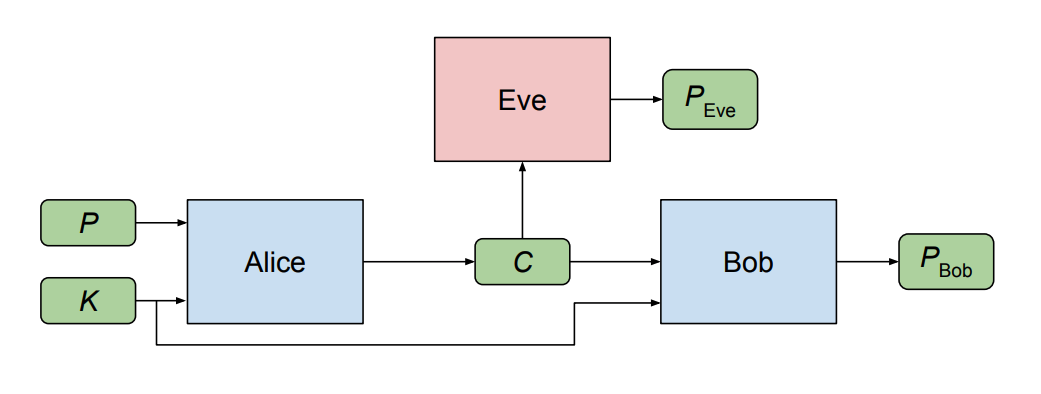
\includegraphics[width=16cm]{../assets/OverviewOfCryptosystem.png}
\caption{Alice, Bob, and Eve networks as symmetric cryptosystem.}
\centering
\end{figure}

The objectives of each of the network is as follows: Eve’s goal is to reconstruct P accurately and therefore minimize the error between P and $P_{Eve}$.  Alice and Bob's goal(s) are to communicate clearly thus to minimize the error between P and $P_{Bob}$ but also to hide their communication from Eve. Eve’s objectives contrast with Alice and Bob’s therefore this problem is a great candidate for adversarial training. Alice and Bob discover a cryptosystem to achieve their objectives.

To review the networks objective in a more formal sense:
\begin{itemize}
\item Alice Network: $C = A(\Theta_{A}, P, K)$
\item Bob Network: $P_{Bob} = B(\Theta_{B}, C, K)$
\item Eve Network: $P_{Eve} = E(\Theta_{E}, C)$
\item L1 distance: $d(P, P^{prime}) = \sum_{i=1, N}|P_{i}-P^{prime}_{i}|$ where N is the length of plaintexts.
\item Bob Reconstruction Error: $L_{B}(\Theta_{A}, \Theta_{B}, P, K) = d(P, B(\Theta_{B}, A(\Theta_{A}, P, K), K))$
\item Eve Reconstruction Error: $L_{E}(\Theta_{A}, \Theta_{E}, P, K) = d(P, E(\Theta_{E}, A(\Theta_{A}, P, K)))$
\item Loss for Alice and Bob: $L_{AB}(\Theta_{A}, \Theta_{B}) = L_{B}(\Theta_{A}, \Theta_{B}, P, K) -  L_{E}(\Theta_{A}, \Theta_{E}, P, K)$ the combination reflects that Alice and Bob want to minimize Bob’s reconstruction error and to maximize the reconstruction error).
\end{itemize}

The network architecture introduced by Adbadi, et al. [1] is known as the Mix and Transform Architecture. All binary encoded plaintext bits are mapped to [-1,1]. Alice and Bob consists of 1 x Fully Connected Layer 2N x 2N where N is the length in bits of the message. The fully connected layer is then followed by 4 x 1D Convolutional Layers with filter sizes [4, 2, 1, 1], input channels [1, 2, 1, 1], output channels[2, 4, 4, 1]. The strides for the 1D convolution by layer are [1, 2, 1, 1]. Note that same convolution is used to all convolutional layers in order to keep input and output diminsions the same. The activation functions used at each layer are the Sigmoid for all layers except final layer which is a Tanh used to bring values back to a range [-1, 1] that can map to binary values. The Eve uses more or less the same architecture except the Fully Connected Layer dimensions are N x 2N where N is the length in bits of the message because only receiving C. It should be noted that P, K are vectors of same size; however, there is no reason that K has to be the same size as P. P and K are generated from uniform distribution and values are mapped from [0,1] to [-1,1] All Network parameters randomly initialized.
The optimization strategy is mini-batch Gradient Descent with the Adam Optimizer. We want to approximate optimal Eve and therefore alternate training between the Alice-Bob and Eve training, training Eve on 2 mini-batches per step in order to give advantage to the adversary.

\section{Experiments}
Initially experiments were performed on the original Mix and Transform Architecture to see if the symmetric cryptosystem would learn and encryption method with non binary values; however, nothing with the original architecture learned to decrypt the P with any success. It is believed that the Mix and Transform Architecture is not an appropiate architecture for a symmetric cryptosystem with anything but binary input. Other experiments were performed with the manipulating the reconstruction errors but nothing performed as well as the original methods provided by the original paper.

\section{Discussion and Analysis}

The original paper Adbadi, et al. [1] reports that training goals typically achieved within 15,000 steps. My implementation in PyTorch confirms these findings.

\begin{figure}[h]
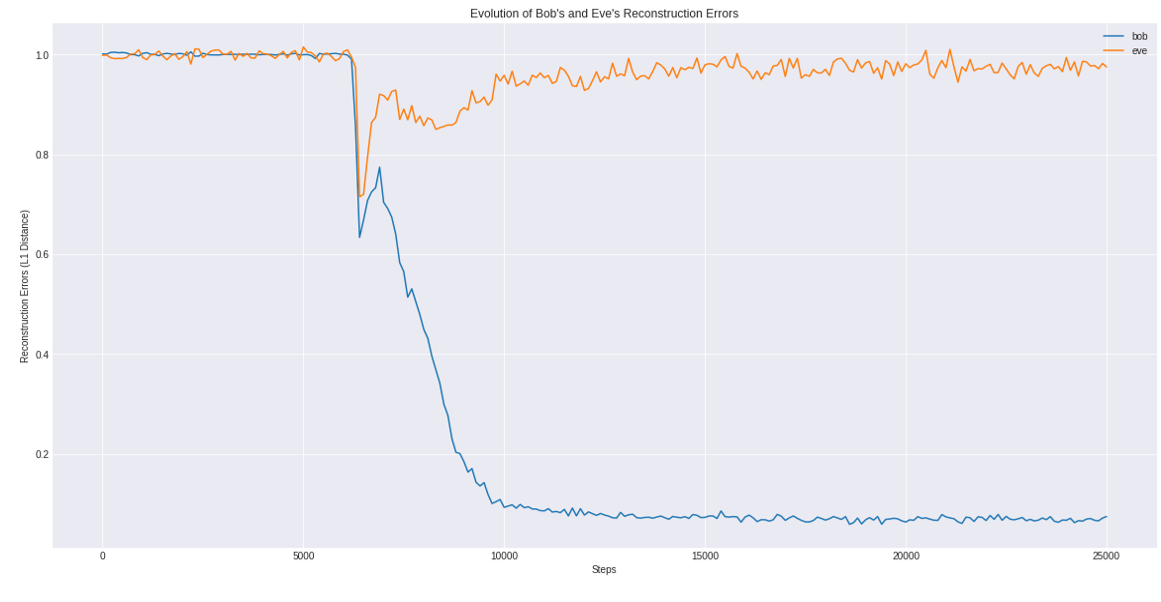
\includegraphics[width=16cm]{../assets/EvolutionOfBobAndEveReconstructionErrors.png}
\caption{Evolution of Bob and Eve Reconstruction Errors.}
\centering
\end{figure}

Bob and Eve accomplish their training goals within approximately 15,000 training steps. It can be observed that Bob's reconstruction error continues to improve while Eve's reconstruction error remains just slightly better than 1 or 2 bits better than random guessing. This shows that Bob's error is being minimized while Eve's error is being maximized.

\begin{figure}[h]
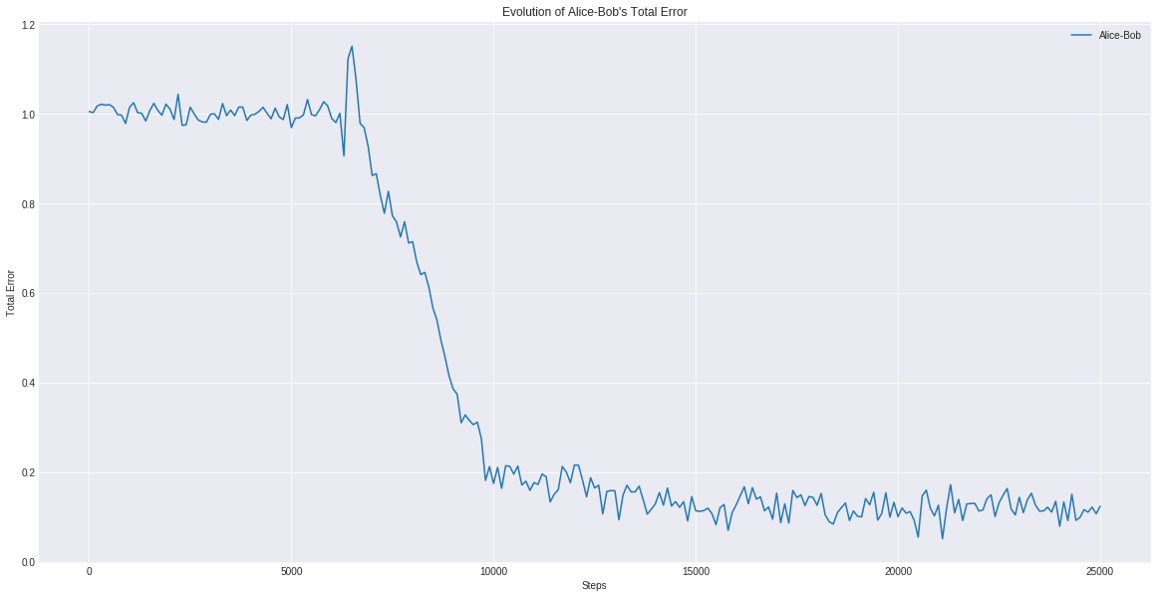
\includegraphics[width=16cm]{../assets/AliceBobTotalError.png}
\caption{Evolution of Alice and Bob Total Error.}
\centering
\end{figure}

In the figure above (Figure 4) it can be observed that Alice and Bob's total training error is improved throughout the training process. These findings were consistent with the results published in the original paper Adbadi, et al. [1].

\section{Conclusion}
The symmetric cryptosystem proposed by Adbadi, et al. [1] shows very promising results for encrypting plaintext messages that are represented in binary. There are several implementation details that prevent this system from having practical application. Working on binary encoded plaintext if the reconstructed plaintext has any bit that is not properly reconstructed it could result in a non valid binary string. In the rehelm of deep learning working with bits does not provide the same computational advantage that it does with classic encryption algorithms. The neural networks proposed in this system could therefore operate over tokenized plaintext rather than binary encoded plaintext with the same computational complexity. In future work to improve the practical application of a deep learning based symmetric cryptosystem could operate over tokenized plain text or even better word embeddings.

\section{Bibliography}

[1] Abadi, Martin, et al., "Learning to Protect Communications
with Adversarial Neural Cryptography". arxiv:1610.06918, October 2016.
\newline

[2] Goodfellow, Ian, et al., "Generative Adversarial Networks". arxiv:1406.2661, June 2014.
\newline

[3] I. Goodfellow, J. Pouget-Abadie, M. Mirza, B. Xu, D. Warde-Farley, S. Ozair, A. Courville, and Y. Bengio, “Generative adversarial nets,”
in Advances in Neural Information Processing Systems, 2014, pp. 2672–2680
\newline

[4] T. Salimans, I. Goodfellow, W. Zaremba, V. Cheung, A. Radford,
and X. Chen, “Improved techniques for training gans,” in Advances
in Neural Information Processing Systems, 2016, pp. 2226–2234
\newline

[5] M. Arjovsky and L. Bottou, “Towards principled methods for
training generative adversarial networks,” NIPS 2016 Workshop
on Adversarial Training, 2016.
\newline

[6] A. Radford, L. Metz, and S. Chintala, “Unsupervised representation
learning with deep convolutional generative adversarial
networks,” in Proceedings of the 5th International Conference on
Learning Representations (ICLR) - workshop track, 2016
\newline

[7] Google Brain, NIPS 2017: Non-targeted Adversarial Attack. https://www.kaggle.com/c/nips-2017-non-targeted-adversarial-attack.
\newline

[8] Greydanus, Sam, "Learning the Enigma with Recurrent Neural Networks", arxiv:1708.07576v2, September 2017.
\newline

[9] Rivest, R. L.; Shamir, A.; Adleman, L. (1978-02-01). "A Method for Obtaining Digital Signatures and Public-key Cryptosystems". Commun. ACM. 21 (2): 120–126. doi:10.1145/359340.359342. ISSN 0001-0782.
\newline

\end{document}